\documentclass{standalone}
\usepackage{tikz}
\usetikzlibrary{patterns, positioning}

\begin{document}
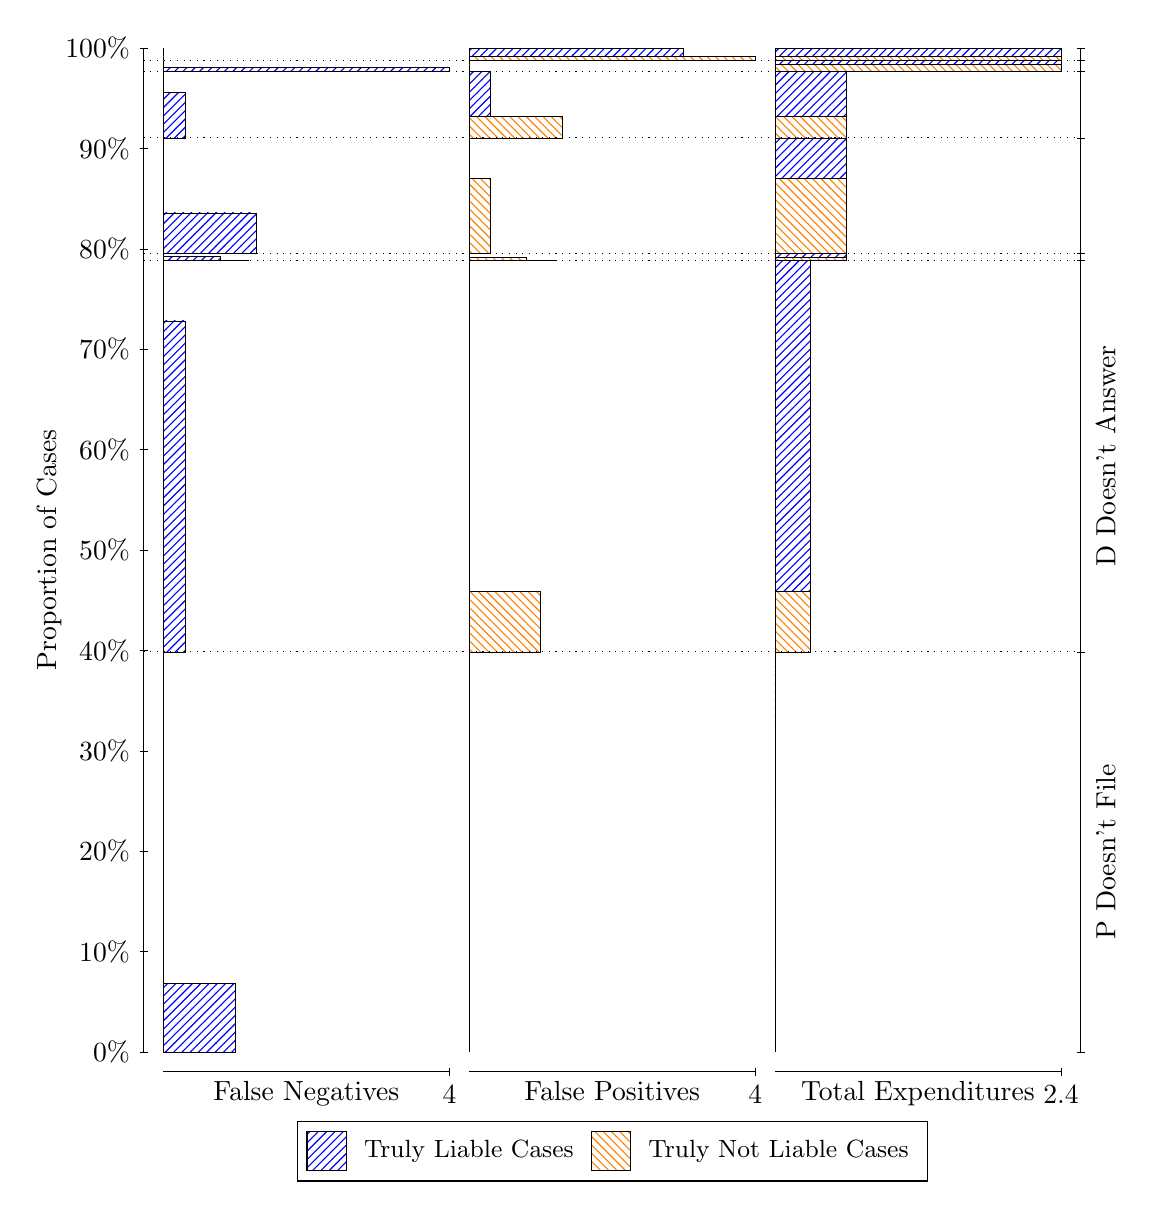
\begin{tikzpicture}
\draw[black, very thin] (1.5,1.75) -- (1.5,14.5);
\node[rotate=90, anchor=center] at (0.3, 8.125) {Proportion of Cases};
\draw[black, very thin] (1.45,1.75) -- (1.55,1.75);
\node[anchor=east] at (1.45, 1.75) {0\%};
\draw[black, very thin] (1.45,3.025) -- (1.55,3.025);
\node[anchor=east] at (1.45, 3.025) {10\%};
\draw[black, very thin] (1.45,4.3) -- (1.55,4.3);
\node[anchor=east] at (1.45, 4.3) {20\%};
\draw[black, very thin] (1.45,5.575) -- (1.55,5.575);
\node[anchor=east] at (1.45, 5.575) {30\%};
\draw[black, very thin] (1.45,6.85) -- (1.55,6.85);
\node[anchor=east] at (1.45, 6.85) {40\%};
\draw[black, very thin] (1.45,8.125) -- (1.55,8.125);
\node[anchor=east] at (1.45, 8.125) {50\%};
\draw[black, very thin] (1.45,9.4) -- (1.55,9.4);
\node[anchor=east] at (1.45, 9.4) {60\%};
\draw[black, very thin] (1.45,10.675) -- (1.55,10.675);
\node[anchor=east] at (1.45, 10.675) {70\%};
\draw[black, very thin] (1.45,11.95) -- (1.55,11.95);
\node[anchor=east] at (1.45, 11.95) {80\%};
\draw[black, very thin] (1.45,13.225) -- (1.55,13.225);
\node[anchor=east] at (1.45, 13.225) {90\%};
\draw[black, very thin] (1.45,14.5) -- (1.55,14.5);
\node[anchor=east] at (1.45, 14.5) {100\%};

\draw[black, very thin] (13.4,1.75) -- (13.4,14.5);
\draw[black, very thin] (13.35,1.75) -- (13.45,1.75);
\node[anchor=west] at (13.35, 1.75) {};
\draw[black, very thin] (13.35,6.8304) -- (13.45,6.8304);
\node[anchor=west] at (13.35, 6.8304) {};
\draw[black, very thin] (13.35,11.806) -- (13.45,11.806);
\node[anchor=west] at (13.35, 11.806) {};
\draw[black, very thin] (13.35,11.89) -- (13.45,11.89);
\node[anchor=west] at (13.35, 11.89) {};
\draw[black, very thin] (13.35,13.36) -- (13.45,13.36);
\node[anchor=west] at (13.35, 13.36) {};
\draw[black, very thin] (13.35,14.204) -- (13.45,14.204);
\node[anchor=west] at (13.35, 14.204) {};
\draw[black, very thin] (13.35,14.343) -- (13.45,14.343);
\node[anchor=west] at (13.35, 14.343) {};
\draw[black, very thin] (13.35,14.5) -- (13.45,14.5);
\node[anchor=west] at (13.35, 14.5) {};

\draw[black, very thin, pattern color=blue, pattern=north east lines] (1.75,1.75) rectangle (2.6583,2.6245);
\draw[black, very thin, pattern color=orange, pattern=north west lines] (1.75,2.6245) rectangle (1.75,6.8304);
\draw[black, very thin, pattern color=blue, pattern=north east lines] (1.75,6.8304) rectangle (2.0225,11.036);
\draw[black, very thin, pattern color=orange, pattern=north west lines] (1.75,11.036) rectangle (1.75,11.806);
\draw[black, very thin, pattern color=blue, pattern=north east lines] (1.75,11.806) rectangle (2.84,11.806);
\draw[black, very thin, pattern color=blue, pattern=north east lines] (1.75,11.806) rectangle (2.7492,11.806);
\draw[black, very thin, pattern color=blue, pattern=north east lines] (1.75,11.806) rectangle (2.6583,11.806);
\draw[black, very thin, pattern color=blue, pattern=north east lines] (1.75,11.806) rectangle (2.5675,11.806);
\draw[black, very thin, pattern color=blue, pattern=north east lines] (1.75,11.806) rectangle (2.5675,11.806);
\draw[black, very thin, pattern color=blue, pattern=north east lines] (1.75,11.806) rectangle (2.4767,11.854);
\draw[black, very thin, pattern color=blue, pattern=north east lines] (1.75,11.854) rectangle (2.3858,11.854);
\draw[black, very thin, pattern color=blue, pattern=north east lines] (1.75,11.854) rectangle (2.295,11.854);
\draw[black, very thin, pattern color=blue, pattern=north east lines] (1.75,11.854) rectangle (2.2042,11.854);
\draw[black, very thin, pattern color=blue, pattern=north east lines] (1.75,11.854) rectangle (2.1133,11.854);
\draw[black, very thin, pattern color=orange, pattern=north west lines] (1.75,11.854) rectangle (1.75,11.89);
\draw[black, very thin, pattern color=blue, pattern=north east lines] (1.75,11.89) rectangle (2.9308,12.407);
\draw[black, very thin, pattern color=orange, pattern=north west lines] (1.75,12.407) rectangle (1.75,13.36);
\draw[black, very thin, pattern color=blue, pattern=north east lines] (1.75,13.36) rectangle (2.0225,13.934);
\draw[black, very thin, pattern color=orange, pattern=north west lines] (1.75,13.934) rectangle (1.75,14.204);
\draw[black, very thin, pattern color=blue, pattern=north east lines] (1.75,14.204) rectangle (5.3833,14.256);
\draw[black, very thin, pattern color=orange, pattern=north west lines] (1.75,14.256) rectangle (1.75,14.343);
\draw[black, very thin, pattern color=orange, pattern=north west lines] (1.75,14.343) rectangle (1.75,14.395);
\draw[black, very thin, pattern color=blue, pattern=north east lines] (1.75,14.395) rectangle (1.75,14.5);
\draw[black, very thin, pattern color=orange, pattern=north west lines] (5.6333,1.75) rectangle (5.6333,5.9559);
\draw[black, very thin, pattern color=blue, pattern=north east lines] (5.6333,5.9559) rectangle (5.6333,6.8304);
\draw[black, very thin, pattern color=orange, pattern=north west lines] (5.6333,6.8304) rectangle (6.5417,7.6006);
\draw[black, very thin, pattern color=blue, pattern=north east lines] (5.6333,7.6006) rectangle (5.6333,11.806);
\draw[black, very thin, pattern color=orange, pattern=north west lines] (5.6333,11.806) rectangle (6.7233,11.806);
\draw[black, very thin, pattern color=orange, pattern=north west lines] (5.6333,11.806) rectangle (6.6325,11.806);
\draw[black, very thin, pattern color=orange, pattern=north west lines] (5.6333,11.806) rectangle (6.5417,11.806);
\draw[black, very thin, pattern color=orange, pattern=north west lines] (5.6333,11.806) rectangle (6.4508,11.806);
\draw[black, very thin, pattern color=orange, pattern=north west lines] (5.6333,11.806) rectangle (6.36,11.843);
\draw[black, very thin, pattern color=orange, pattern=north west lines] (5.6333,11.843) rectangle (6.2692,11.843);
\draw[black, very thin, pattern color=orange, pattern=north west lines] (5.6333,11.843) rectangle (6.1783,11.843);
\draw[black, very thin, pattern color=orange, pattern=north west lines] (5.6333,11.843) rectangle (6.0875,11.843);
\draw[black, very thin, pattern color=orange, pattern=north west lines] (5.6333,11.843) rectangle (5.9967,11.843);
\draw[black, very thin, pattern color=blue, pattern=north east lines] (5.6333,11.843) rectangle (5.815,11.843);
\draw[black, very thin, pattern color=blue, pattern=north east lines] (5.6333,11.843) rectangle (5.7242,11.843);
\draw[black, very thin, pattern color=blue, pattern=north east lines] (5.6333,11.843) rectangle (5.6333,11.89);
\draw[black, very thin, pattern color=orange, pattern=north west lines] (5.6333,11.89) rectangle (5.9058,12.844);
\draw[black, very thin, pattern color=blue, pattern=north east lines] (5.6333,12.844) rectangle (5.6333,13.36);
\draw[black, very thin, pattern color=orange, pattern=north west lines] (5.6333,13.36) rectangle (6.8142,13.63);
\draw[black, very thin, pattern color=blue, pattern=north east lines] (5.6333,13.63) rectangle (5.9058,14.204);
\draw[black, very thin, pattern color=orange, pattern=north west lines] (5.6333,14.204) rectangle (5.6333,14.292);
\draw[black, very thin, pattern color=blue, pattern=north east lines] (5.6333,14.292) rectangle (5.6333,14.343);
\draw[black, very thin, pattern color=orange, pattern=north west lines] (5.6333,14.343) rectangle (9.2667,14.395);
\draw[black, very thin, pattern color=blue, pattern=north east lines] (5.6333,14.395) rectangle (8.3583,14.5);
\draw[black, very thin, pattern color=orange, pattern=north west lines] (9.5167,1.75) rectangle (9.5167,5.9559);
\draw[black, very thin, pattern color=blue, pattern=north east lines] (9.5167,5.9559) rectangle (9.5167,6.8304);
\draw[black, very thin, pattern color=orange, pattern=north west lines] (9.5167,6.8304) rectangle (9.9708,7.6006);
\draw[black, very thin, pattern color=blue, pattern=north east lines] (9.5167,7.6006) rectangle (9.9708,11.806);
\draw[black, very thin, pattern color=orange, pattern=north west lines] (9.5167,11.806) rectangle (10.425,11.843);
\draw[black, very thin, pattern color=blue, pattern=north east lines] (9.5167,11.843) rectangle (10.425,11.89);
\draw[black, very thin, pattern color=orange, pattern=north west lines] (9.5167,11.89) rectangle (10.425,11.89);
\draw[black, very thin, pattern color=blue, pattern=north east lines] (9.5167,11.89) rectangle (10.425,11.89);
\draw[black, very thin, pattern color=orange, pattern=north west lines] (9.5167,11.89) rectangle (10.425,11.89);
\draw[black, very thin, pattern color=blue, pattern=north east lines] (9.5167,11.89) rectangle (10.425,11.89);
\draw[black, very thin, pattern color=orange, pattern=north west lines] (9.5167,11.89) rectangle (10.425,12.844);
\draw[black, very thin, pattern color=blue, pattern=north east lines] (9.5167,12.844) rectangle (10.425,13.36);
\draw[black, very thin, pattern color=orange, pattern=north west lines] (9.5167,13.36) rectangle (10.425,13.63);
\draw[black, very thin, pattern color=blue, pattern=north east lines] (9.5167,13.63) rectangle (10.425,14.204);
\draw[black, very thin, pattern color=orange, pattern=north west lines] (9.5167,14.204) rectangle (13.15,14.292);
\draw[black, very thin, pattern color=blue, pattern=north east lines] (9.5167,14.292) rectangle (13.15,14.343);
\draw[black, very thin, pattern color=orange, pattern=north west lines] (9.5167,14.343) rectangle (13.15,14.395);
\draw[black, very thin, pattern color=blue, pattern=north east lines] (9.5167,14.395) rectangle (13.15,14.5);
\draw[black, dotted] (1.5,6.8304) -- (13.4,6.8304);
\draw[black, dotted] (1.5,11.806) -- (13.4,11.806);
\draw[black, dotted] (1.5,11.89) -- (13.4,11.89);
\draw[black, dotted] (1.5,13.36) -- (13.4,13.36);
\draw[black, dotted] (1.5,14.204) -- (13.4,14.204);
\draw[black, dotted] (1.5,14.343) -- (13.4,14.343);
\draw[black, very thin] (1.75,1.5) -- (5.3833,1.5);
\node[anchor=north] at (3.5667, 1.5) {False Negatives};
\draw[black, very thin] (5.3833,1.45) -- (5.3833,1.55);
\node[anchor=north] at (5.3833, 1.45) {4};

\draw[black, very thin] (5.6333,1.5) -- (9.2667,1.5);
\node[anchor=north] at (7.45, 1.5) {False Positives};
\draw[black, very thin] (9.2667,1.45) -- (9.2667,1.55);
\node[anchor=north] at (9.2667, 1.45) {4};

\draw[black, very thin] (9.5167,1.5) -- (13.15,1.5);
\node[anchor=north] at (11.333, 1.5) {Total Expenditures};
\draw[black, very thin] (13.15,1.45) -- (13.15,1.55);
\node[anchor=north] at (13.15, 1.45) {2.4};

\node[black, centered, rotate=90] at (13.72, 4.2902) {P Doesn't File};
\node[black, centered, rotate=90] at (13.72, 9.3182) {D Doesn't Answer};






\draw (7.449999999999999,1.5) node[draw=none] (baseCoordinate) {};
\begin{scope}[align=center]
        \matrix[scale=0.5, draw=black, below=0.5cm of baseCoordinate, nodes={draw}, column sep=0.1cm]{
            \node[rectangle, draw, minimum width=0.5cm, minimum height=0.5cm, pattern=north east lines, pattern color=blue] {}; &
            \node[draw=none, font=\small] (B) {Truly Liable Cases}; &
            \node[rectangle, draw, minimum width=0.5cm, minimum height=0.5cm, pattern=north west lines, pattern color=orange] {}; &
            \node[draw=none, font=\small] (B) {Truly Not Liable Cases}; \\
            };
\end{scope}

\end{tikzpicture}
\end{document}